\newpage
\part{Постановка задачи}
\section{Назначение и общий вид манипулятора}
Целью данной курсовой работы ставится проектирование одного из двух
приводов манипулятора, устанавливаемых на малых спутниках съемки Земли (рис. \ref{sattelite_general_view}).
Манипулятор представляет собой двухзвенный электроприводной механизм,
предназначенный для скоростного наведения оптических камер.
Задачей манипулятора является организация перенацеливания камеры в заданное положение.

\begin{figure}[h!]
\centering
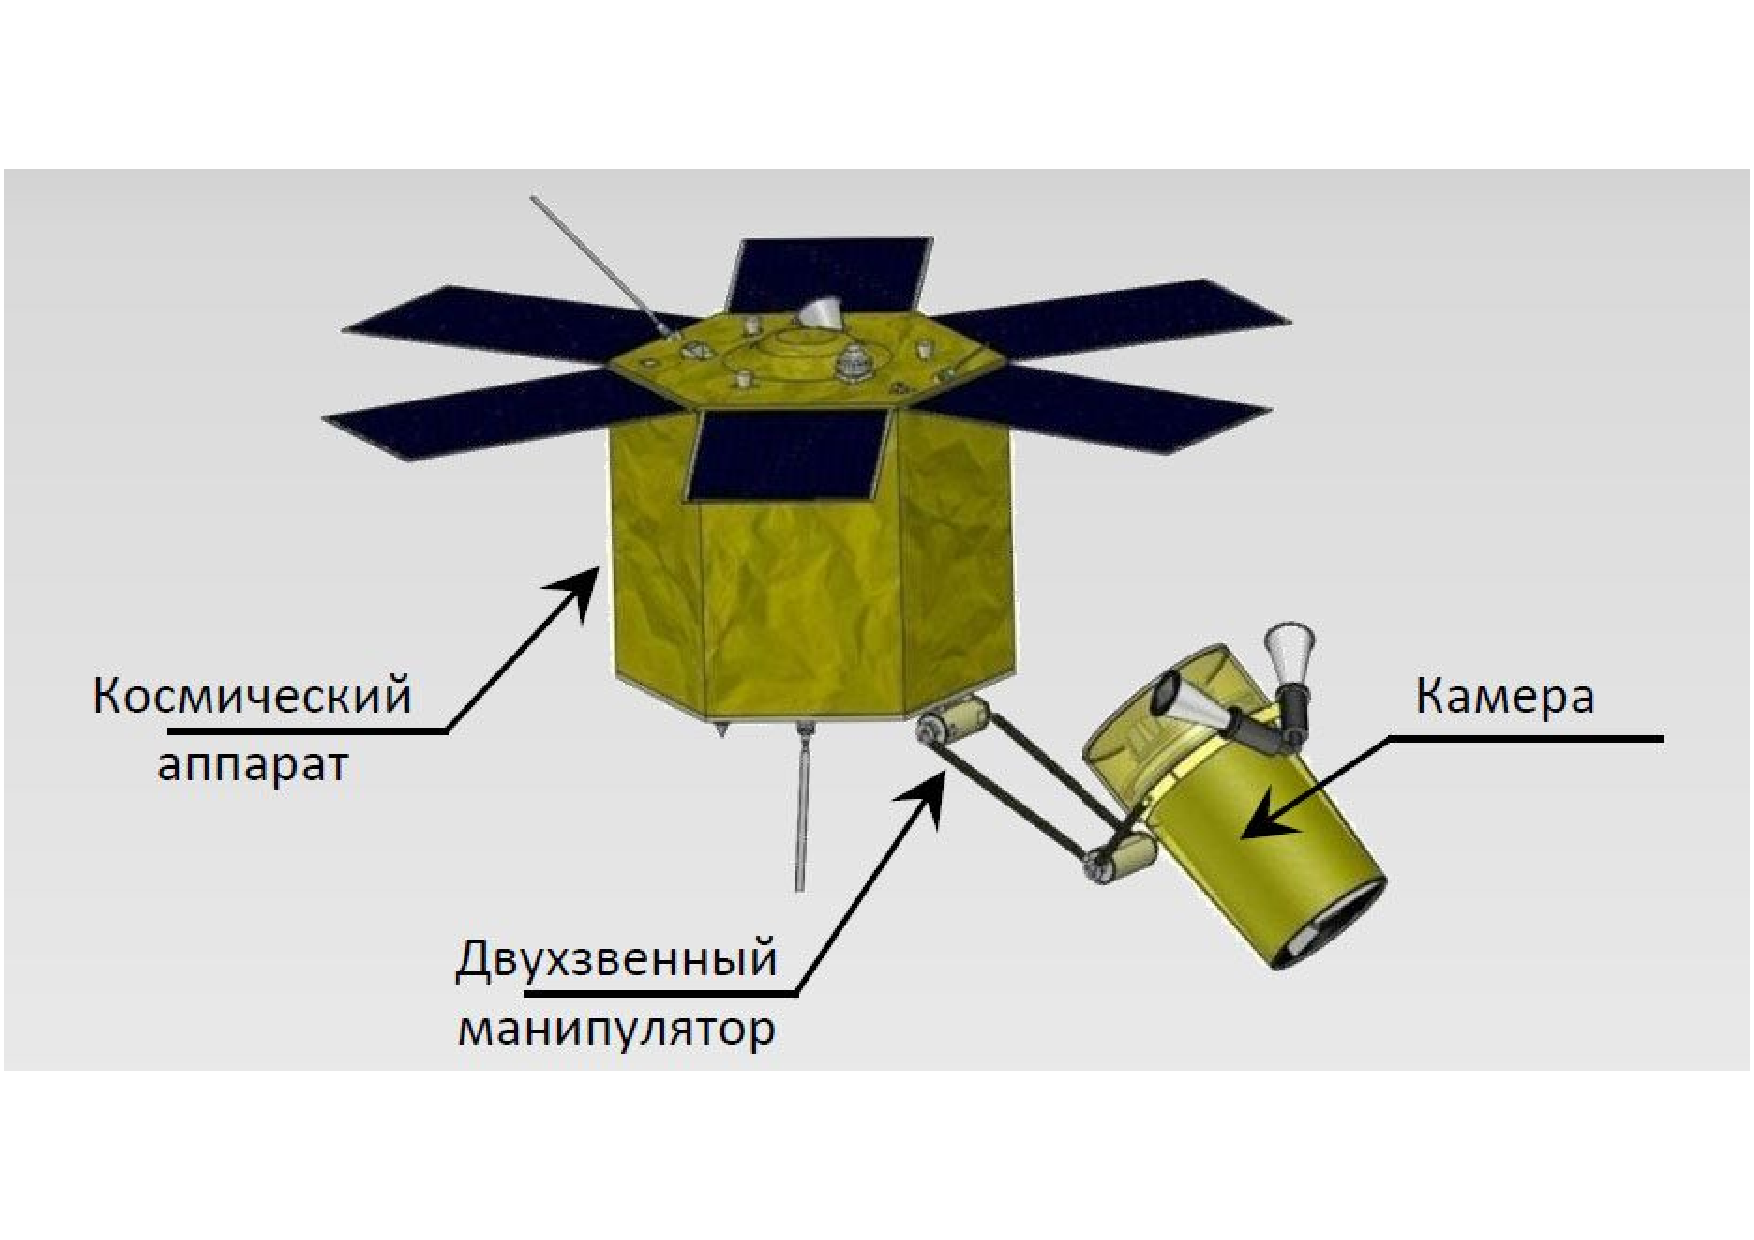
\includegraphics[width=\textwidth, keepaspectratio, clip=true, trim=0mm 25mm 0mm 25mm]{./src/pictures/sattelite_3d_images/general_view}
\caption{Манипулятор наведения камеры малого КА}
\label{sattelite_general_view}
\end{figure}

Программные движения манипулятора осуществляются с помощью двух электроприводных блоков,
обеспечивающих поворот камеры в одной плоскости (в плоскости перпендикулярной
вектору движения космического аппарата по орбите).

В данный момент манипуляторы подобного рода на спутниках широко востребованы
в областях картографирования, планировки территорий, образовательных,
разведывательных и военных целях, метеорологии и т.п.

К подобным манипуляторам предъявляют высокие требования по точности,
надежности, массе, габаритам.

В качестве объекта проектирования был выбран малый привод, непосредственно вращающий камеру.

\section{Описание объекта управления}
Проектируемый привод установлен на малом спутнике Земли и представляет собой
исполнительный элемент системы дистанционного зондирования Земли (далее - ДЗЗ).
Объектом управления является специальная камера, предназначенная для создания
снимком поверхности Земли высокой четкости, оборудована двумя звёздными
датчиками для ориентации в пространстве и находящаяся внутри корпуса
экранно-вакуумной теплоизоляции (далее - ЭВТИ).

Общая масса камеры и ее навесных элементов: 60.5 кг. С учетом запаса, выберем
массу объекта управления манипулятора: 80 кг.
Расстояние от оси привода до центра масс камеры: 400 мм (с учетом запаса
на более габаритную камеру и запаса на ускорение камеры);
Собственный момент инерции объекта управления вокруг оси, параллельной оси привода:
$$
    J_{pl} = 2.84 kg \cdot m^2
$$

Момент инерции относительно оси привода:
$$
    15.7 kg \cdot m^2
$$

%\section{Требуемые параметры перенацеливания приводных блоков}

\section{Требуемые параметры привода}

\begin{tabular}{|l|c|l|}
\hline
Параметр                                    & Обозначение      & Значение                   \\
\hline
Напряжение питания                          & $U_1$            & 24В                        \\
Шаг единичного углового перемещения нагрузки& $q_d$            & $ \le 1' $                 \\
Ресурс                                      &                  & 30 000 ч.                  \\
Диапазон углового перенацеливания нагрузки  & $q_{max}$        & $[-135^\circ, 135^\circ] $ \\
Максимальная угловая скорость нагрузки      & $\dot{q}_{max}$  & $1.73$ рад / c             \\
Максимальное ускорение нагрузки             & $\ddot{q}_{max}$ & $0.872$ рад /$c^2$         \\
Момент инерции нагрузки                     & $J_{pl}$         & $3 kg \cdot m^2 $          \\
\hline
\end{tabular}

\endinput

